\documentclass[a4paper,14pt]{extarticle}
\usepackage{geometry}
\usepackage[utf8]{inputenc}
\usepackage{csquotes}
\usepackage[T1]{fontenc}
\usepackage[main=english, russian]{babel}   % use russian via \foreignlanguage{russian}{}
\usepackage{amsmath}
\usepackage{amsthm}
\usepackage{amssymb}
\usepackage{fancyhdr}
\usepackage{setspace}
\usepackage{graphicx}
\usepackage{colortbl}
\usepackage{tikz}
\usepackage{pgf}
\usepackage{subcaption}
\usepackage{listings}
\usepackage{indentfirst}
\usepackage[colorlinks,citecolor=blue,linkcolor=blue,bookmarks=false,hypertexnames=true, urlcolor=blue]{hyperref} 
\usepackage{indentfirst}
\usepackage{mathtools}
\usepackage{booktabs}
\usepackage[flushleft]{threeparttable}
\usepackage{tablefootnote}

\usepackage{chngcntr}
\counterwithin{equation}{section}
\counterwithin{table}{section}
\counterwithin{figure}{section}

% \graphicspath{{graphics/}}

% add bibliography using biblatex
% if if all authors in bibliography are needed => add 'maxbibnames=99' in []:
\usepackage[backend=bibtex, citestyle=authoryear]{biblatex}
\addbibresource{bibliography.bib}
\DeclareFieldFormat{labelnumberwidth}{#1\adddot}
\setlength{\biblabelsep}{5pt}
 

\geometry{left=2.5cm} % left margin
\geometry{right=1.5cm} % right margin
\geometry{top=1.5cm} % top margin
\geometry{bottom=1.5cm} % bottom margin
\renewcommand{\baselinestretch}{1.5} % line spacing


\renewcommand{\theenumi}{\arabic{enumi}} % Make all enumerations to be in form digit.digit
\renewcommand{\labelenumi}{\arabic{enumi}}
\renewcommand{\theenumii}{.\arabic{enumii}}
\renewcommand{\labelenumii}{\arabic{enumi}.\arabic{enumii}.}
\renewcommand{\theenumiii}{.\arabic{enumiii}}
\renewcommand{\labelenumiii}{\arabic{enumi}.\arabic{enumii}.\arabic{enumiii}.}

\begin{document}
\begin{titlepage}
	\newpage

	{\setstretch{1.0}
		\begin{center}
			Federal State Autonomous Educational Institution for Higher Education
			National Research University Higher School of Economics
			\\
			\bigskip
			Information Security \\
		\end{center}
	}

	\vspace{8em}

	\begin{center}
		{\Large BACHELOR'S THESIS}\\
		\textsc{\textbf{
				Research project
				\linebreak
				"Hybrid Fuzzing of the PyTorch Framework"}}
	\end{center}

	\vspace{4em}

	{\setstretch{1.0}
		\hfill\parbox{16cm}{
			\hspace*{5cm}\hspace*{-5cm}Prepared by the student of group 191, 4th year of study,\\
			Larionov-Trichkine Theodor Arsenij\\

			\hspace*{5cm}\hspace*{-5cm}Supervisor:\\
			PhD, Petrenko Alexander Konstantinovich
			\\
		}
	}

	\vspace{\fill}

	\begin{center}
		Moscow 2023
	\end{center}

\end{titlepage}
 % title page
\newpage

{
	\hypersetup{linkcolor=black}
	\tableofcontents
}

\newpage
\section*{Annotation}
\addcontentsline{toc}{section}{Annotation} % add Annotation to Table of Contents

Your annotation in English.

\section*{\foreignlanguage{russian}{Аннотация}} % this is how to use russian
\foreignlanguage{russian}{
	Ваша аннотация на русском языке.
}

\section*{Keywords}
NLP, CV, DL, ML, RL, GAN,
\pagebreak

\section{Introduction}

\subsection{Citing}

In this template you have to insert all your references in a special file
called "bibliography.bib". It should be inserted in a special BibTeX format.
It can be found easily via Google Scholar -> quotation sign -> BibTeX. You can find how it looks in ".bib" file.

After you have inserted your BibTeX citation into the ".bib" file, you can cite it in this document using \cite{vaswani2017}.

Or you can cite it in the following way: \cite{kim2020code}.

\subsection{Graphs}

Graph \ref{fig:by_epochs} shows the results of the experiment.

\begin{figure}[h!]
	\centering
	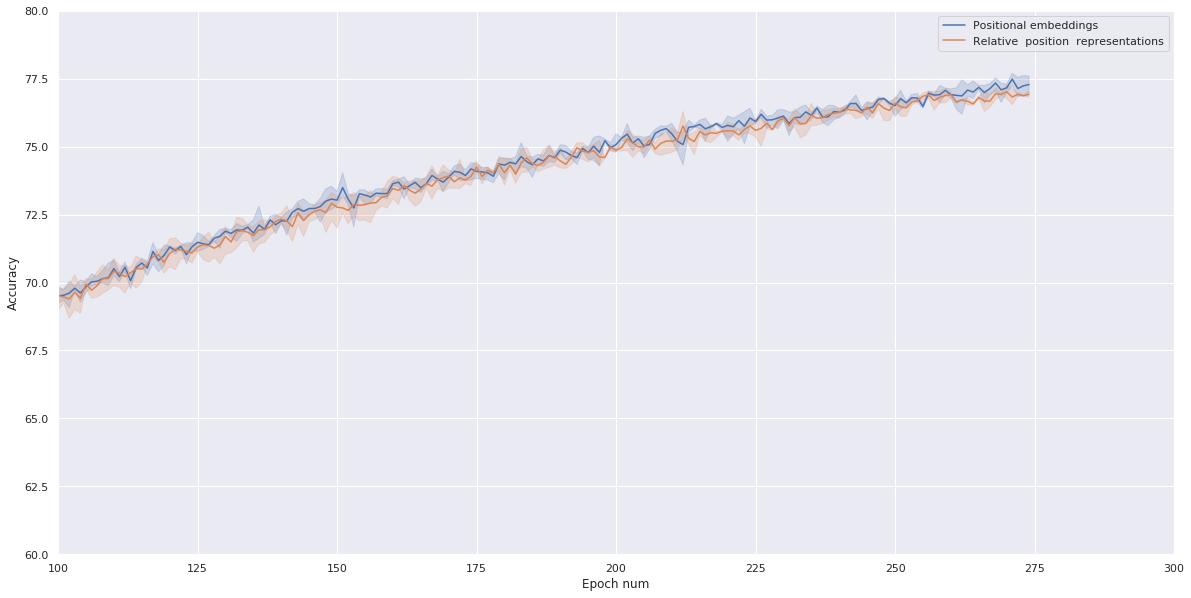
\includegraphics[width=1\textwidth]{graph2.png}
	\caption{Graph sample}
	\label{fig:by_epochs}
\end{figure}

\pagebreak

\subsection{Tables}

\begin{table}[htbp]
	\caption{Table example}
	\label{table:long_epochs}
	\footnotesize
	\centering
	\begin{tabular}{lrrrrrrrr}
		\toprule
		              & \multicolumn{3}{c}{$\mathsf{Val}$} &
		\multicolumn{3}{c}{$\mathsf{Test}$}                                                                                                                                              \\
		\cmidrule(lr){2-4} \cmidrule(l){5-7}
		{}            & $\mathsf{Prec}$                    & $\mathsf{Rec}$ & $\mathsf{F1}$ & $\mathsf{Prec}$ & $\mathsf{Rec}$ & $\mathsf{F1}$ & $\mathsf{nodes}$ & $\mathsf{subtokens}$ \\
		\midrule
		run \#1       & 0.4894                             & 0.3775         & 0.4263        & 0.4824          & 0.3683         & 0.4177        & 10029            & 179                  \\
		run \#2       & 0.4887                             & 0.3739         & 0.4237        & 0.4891          & 0.3724         & 0.4228        & 10039            & 177                  \\
		run \#3       & 0.4820                             & 0.3751         & 0.4219        & 0.4838          & 0.3677         & 0.4178        & 10037            & 180                  \\
		\midrule
		\bf{mean}     & \bf{0.4867}                        & \bf{0.3755}    & \bf{0.4239}   & \bf{ 0.4851}    & \bf{0.3695}    & \bf{0.4195}                                             \\
		\bf{variance} & 0.0041                             & 0.0019         & 0.0022        & 0.0036          & 0.0025         & 0.0029                                                  \\
		\bottomrule
	\end{tabular}
\end{table}


\newpage

% 1 command to write all citations into the References
\printbibliography[heading=bibintoc]   % [] are for appearing in Table of Contents

\end{document}
